\documentclass[12pt]{article}

\usepackage{sbc-template}

\usepackage{graphicx,url}

\usepackage[brazil]{babel}   
%\usepackage[latin1]{inputenc}  
\usepackage[utf8]{inputenc}  
% UTF-8 encoding is recommended by ShareLaTex

\usepackage{listings}
\usepackage{xcolor}
\lstset { %
    language=C,
    %backgroundcolor=\color{black!5}, % set backgroundcolor
    basicstyle=\footnotesize,% basic font setting
}

\usepackage{todonotes}
     
\sloppy

\title{Trabalho Prático I}

\author{Hariel D. Giacomuzzi\inst{1}, Leonardo G. Carvalho\inst{1}, Matheus S. Redecker\inst{1}}

\address{Pontifícia Universidade Católica do Rio Grande do Sul (PUCRS), \\ Avenida Ipiranga, 6681. Prédio 32, CEP 90619-900. Porto Alegre, RS-Brasil 
  \email{\{hariel.dias, leonardo.gubert, matheus.redecker\}@acad.pucrs.br}
}
\begin{document} 

\maketitle
\section{Algoritmos de Escalonamento}
O objetivo deste trabalho é alterar a forma de escalonamento do Sistema Operacional HellfireOS\footnote{https://github.com/sjohann81/hellfireos}. O algoritmo sendo utilizado por padrão é o Rate Monotonic (RM), e o algoritmo de utilizado neste trabalho será o Earliest Deadline First (EDF). Após a implementação do algoritmo iremos comparar os resultados obtidos no sistema com os obtidos utilizando o simulador Cheddar\footnote{http://beru.univ-brest.fr/~singhoff/cheddar/}. Vale ressaltar que em ambos os tipos de escalonamento estamos assumindo que o \textit{deadline} da tarefa é igual ao seu período.

\subsection{Rate-Monotonic}
O algoritmo de Rate-Monotonic (RM) é um algoritmo de escalonamento utilizado em sistemas de tempo-real que leva em consideração a duração das tarefas do sistema. Quanto \textbf{menor} a duração da tarefa, \textbf{maior} será sua prioridade para ser escalonada.

\subsection{Earliest Deadline First}
O algoritmo EDF tem como objetivo priorizar a execução de tarefas do sistema cujo \newline \textit{deadline} está mais perto de expirar. Este algoritmo tem a capacidade de utilizar até 100\% da capacidade de processamento do sistema em que se encontra. A implementação dele no ambiente do HellfireOS pode ser observada abaixo.

\begin{lstlisting}[showstringspaces=false]
/**
 *  Sort the queue of real time tasks by order of deadline,
 * in order to implement the EDF algorithm.
 **/
static void sort_queue_by_deadline(void)
{
    int32_t i, j, cnt;
    struct tcb_entry *e1, *e2;
    
    cnt = hf_queue_count(krnl_rt_queue);
    for (i = 0; i < cnt-1; i++){
        for (j = i + 1; j < cnt; j++){
            e1 = hf_queue_get(krnl_rt_queue, i);
            e2 = hf_queue_get(krnl_rt_queue, j);
            if (e1->deadline_rem > e2->deadline_rem)
                if (hf_queue_swap(krnl_rt_queue, i, j)) panic(PANIC_CANT_SWAP);
        }
    }
}

int32_t sched_edf(void)
{
    int32_t i, k;
    uint16_t id = 0;
    
    k = hf_queue_count(krnl_rt_queue);
    if (k == 0)
        return 0;
    
    sort_rt_queue_by_deadline();
    
    for (i = 0; i < k; i++){
        krnl_task = hf_queue_remhead(krnl_rt_queue);
        if (!krnl_task) panic(PANIC_NO_TASKS_RT);
        if (hf_queue_addtail(krnl_rt_queue, krnl_task))
            panic(PANIC_CANT_PLACE_RT);
        if (krnl_task->state != TASK_BLOCKED &&
            krnl_task->capacity_rem > 0 && !id){
            id = krnl_task->id;
            if (--krnl_task->capacity_rem == 0)
                krnl_task->rtjobs++;
        }
        if (--krnl_task->deadline_rem == 0){
            krnl_task->deadline_rem = krnl_task->period;
            if (krnl_task->capacity_rem > 0) krnl_task->deadline_misses++;
            krnl_task->capacity_rem = krnl_task->capacity;
        }
    }
    
    if (id){
        krnl_task = &krnl_tcb[id];
        return id;
    }else{
        krnl_task = &krnl_tcb[0];
        return 0;
    }
}
\end{lstlisting}


\section{Aplicações sintéticas}
Para realizarmos a análise dos algoritmos, criamos  três aplicações sintéticas. As aplicações sintéticas são utilizadas apenas para simular o comportamento de tarefas reais em um Sistema Operacional, porém não realizam nenhuma tarefa significativa. As mesmas tarefas sintéticas foram modeladas na ferramenta de simulação Cheddar, com parâmetros apresentados na Tabela~\ref{tab:param}. Para cada aplicação apresentaremos uma descrição do motivo da utilização desses parâmetros, o código usado para executar a aplicação no HellfireOS e uma amostra de escalonamento gerada no Cheddar e outra no Kprofiler. No Chedder o escalonamento para os dois algoritmos estão na mesma imagem e aparecem de forma intercalada, sendo primeiro o escalonamento da tarefa utilizando EDF e em seguida a mesma tarefa sendo escalonada com RM.

\begin{table}[h]
\centering
\caption{Especificação das Tarefas}
\label{tab:param}
\begin{tabular}{|c|c|c|c|c|c|}
\hline
\textbf{Aplicação} & \multicolumn{1}{l|}{\textbf{Tarefa}} & \textbf{Periodo} & \textbf{Capacidade} & \textbf{Deadline} & \textbf{Utilização} \\ \hline
\textbf{1}         &                                      &                  &                     &                   & 0,6483              \\ \hline
                   & \textbf{T1}                          & 15               & 2                   & 15                & 0,1333              \\ \hline
                   & \textbf{T2}                          & 30               & 1                   & 30                & 0,0333              \\ \hline
                   & \textbf{T3}                          & 20               & 2                   & 20                & 0,1                 \\ \hline
                   & \textbf{T4}                          & 24               & 4                   & 24                & 0,1667              \\ \hline
                   & \textbf{T5}                          & 100              & 9                   & 100               & 0,09                \\ \hline
                   & \textbf{T6}                          & 40               & 5                   & 40                & 0,125               \\ \hline
2                  &                                      &                  &                     &                   & 0,9011              \\ \hline
                   & \textbf{T1}                          & 12               & 1                   & 12                & 0,0833              \\ \hline
                   & \textbf{T2}                          & 10               & 3                   & 10                & 0,3                 \\ \hline
                   & \textbf{T3}                          & 15               & 1                   & 15                & 0,0667              \\ \hline
                   & \textbf{T4}                          & 17               & 2                   & 17                & 0,1177              \\ \hline
                   & \textbf{T5}                          & 30               & 5                   & 30                & 0,1667              \\ \hline
                   & \textbf{T6}                          & 24               & 4                   & 24                & 0,1667              \\ \hline
3                  &                                      &                  &                     &                   & 1                   \\ \hline
                   & \textbf{T1}                          & 10               & 2                   & 10                & 0,2                 \\ \hline
                   & \textbf{T2}                          & 30               & 5                   & 30                & 0,1667              \\ \hline
                   & \textbf{T3}                          & 50               & 10                  & 50                & 0,2                 \\ \hline
                   & \textbf{T4}                          & 30               & 6                   & 30                & 0,2                 \\ \hline
                   & \textbf{T5}                          & 30               & 1                   & 30                & 0,0333              \\ \hline
                   & \textbf{T6}                          & 40               & 8                   & 40                & 0,2                 \\ \hline
\end{tabular}
\end{table}


\subsection{Aplicação 1}
A aplicação 1 foi pensada para ter uma utilização que os dois algoritmos consigam executar normalmente, e é o que acontece. Com uma utilização de aproximadamente 65\% os dois algoritmos escalonam fácil esse conjunto de tarefas.
 
\subsubsection{Código} 
\begin{lstlisting}[showstringspaces=false]
#include <hellfire.h>

void task(void){
	for(;;){
		printf("task %d \n", hf_selfid());		
		delay_ms(200);
	}
}
void app_main(void){
	hf_spawn(task, 15, 2, 15, "task 1", 1024);
	hf_spawn(task, 30, 1, 30, "task 2", 1024);
	hf_spawn(task, 20, 2, 20, "task 3", 1024);
	hf_spawn(task, 24, 4, 24, "task 4", 1024);
	hf_spawn(task, 100, 9, 100, "task 5", 1024);
	hf_spawn(task, 40, 5, 40, "task 6", 1024);
}
\end{lstlisting}

\subsubsection{Amostra do Escalonamento}

A Figura~\ref{fig:app1Hell} ilustra uma amostra do escalonamento gerado pelo HellfireOS, a Figura~\ref{fig:app1Chedder} mostra o escalonamento de dois processadores, um utilizando EDF e o outro RM. 

\begin{figure}[ht]
\centering
\caption{Aplicação 1 HellfireOS}
\label{fig:app1Hell}
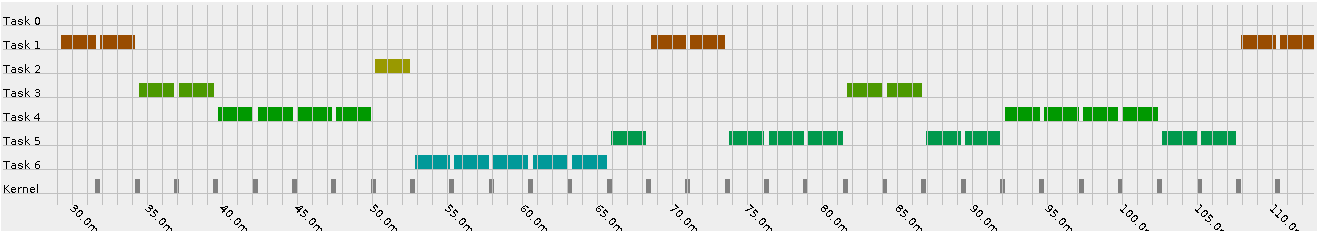
\includegraphics[width=\columnwidth]{fig/app1HellSc.png}
\end{figure}

\begin{figure}[ht]
\centering
\caption{Aplicação 1 Cheddar}
\label{fig:app1Chedder}
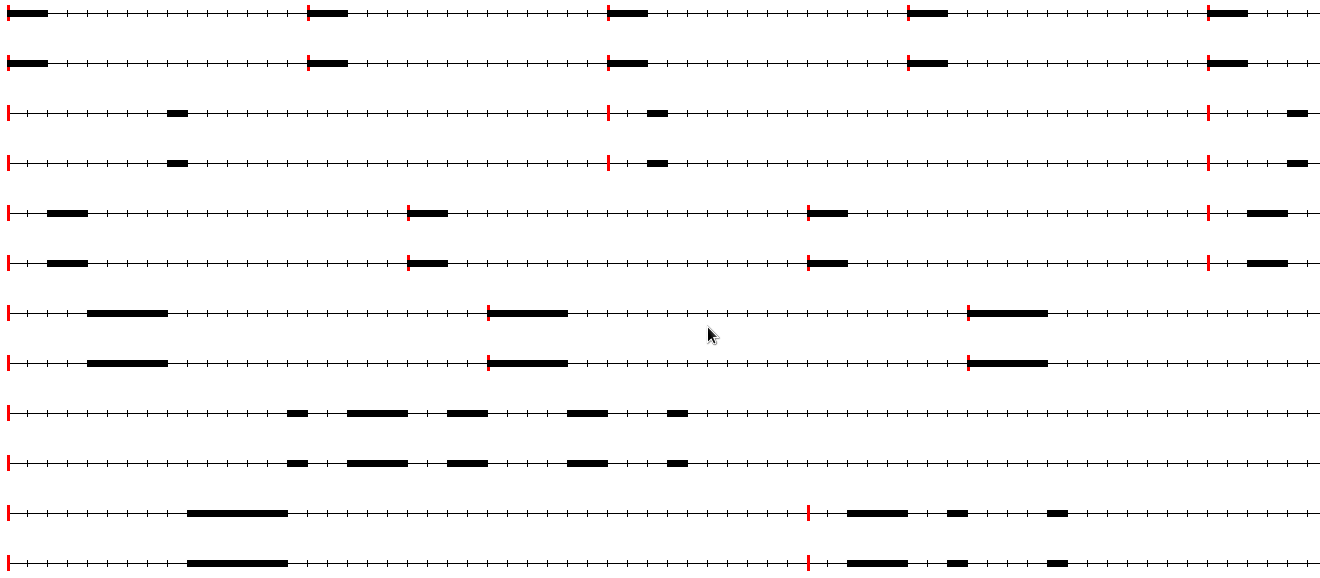
\includegraphics[width=\columnwidth]{fig/app1CheSc.png}
\end{figure}

\subsection{Aplicação 2}
A aplicação 2 foi pensada para que a utilização ultrapasse 85\%. Com o intuito de avaliar se os dois algoritmos continuam escalonando normalmente. A partir da analise dos escalonamentos, podemos notar que o algoritmo RM tem \textit{deadlines} perdidos na tarefa 5, e por isso não consegue ser escalonável. Já o EDF escalona todas as tarefas sem perdas de \textit{deadline}.

\subsubsection{Código} 
\begin{lstlisting}[showstringspaces=false]
#include <hellfire.h>

void task(void){
	for(;;){
		printf("task %d \n", hf_selfid());		
		delay_ms(200);
	}
}
void app_main(void){
	hf_spawn(task, 12, 1, 12, "task 1", 1024);
	hf_spawn(task, 10, 3, 10, "task 2", 1024);
	hf_spawn(task, 15, 1, 15, "task 3", 1024);
	hf_spawn(task, 17, 2, 17, "task 4", 1024);
	hf_spawn(task, 30, 5, 30, "task 5", 1024);
	hf_spawn(task, 24, 4, 24, "task 6", 1024);
}
\end{lstlisting}

\subsubsection{Amostra do Escalonamento}

A Figura~\ref{fig:app2Hell} ilustra uma amostra do escalonamento gerado pelo HellfireOS com o algoritmo de RM e a Figura~\ref{fig:app2HellEDF} o escalonamento utilizando EDF, já a Figura~\ref{fig:app2Chedder} mostra o escalonamento de dois processadores, um utilizando EDF e o outro RM. 

\begin{figure}[ht]
\centering
\caption{Aplicação 2 HellfireOS com algoritmo de RM}
\label{fig:app2Hell}
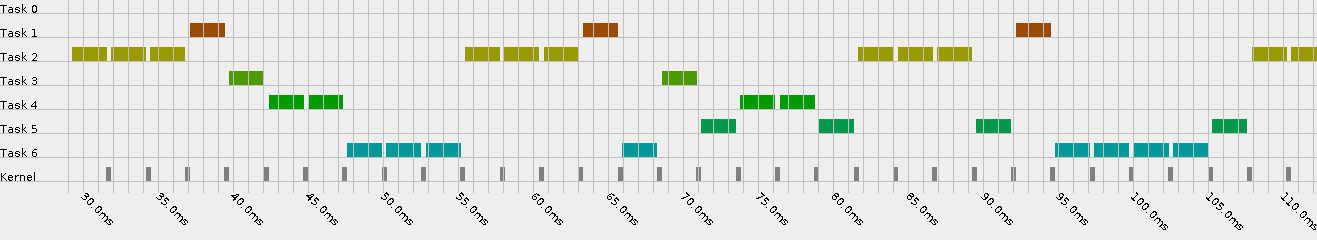
\includegraphics[width=\columnwidth]{fig/app2HellSc.png}
\end{figure}

\begin{figure}[ht]
\centering
\caption{Aplicação 2 HellfireOS com algoritmo de EDF}
\label{fig:app2HellEDF}
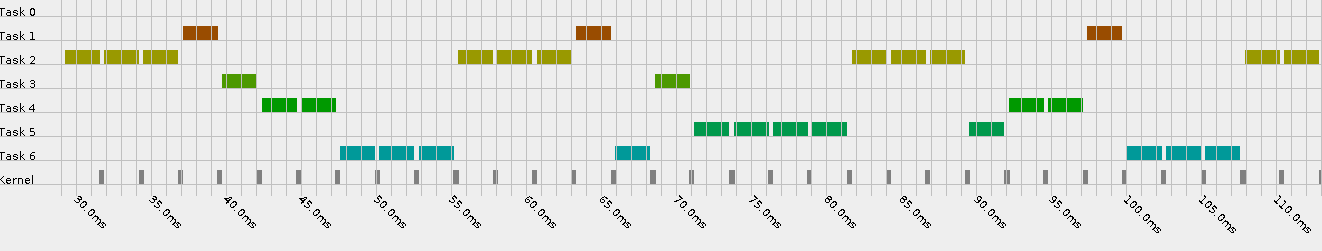
\includegraphics[width=\columnwidth]{fig/app2HellScEDF.png}
\end{figure}

\begin{figure}[ht]
\centering
\caption{Aplicação 2 Cheddar}
\label{fig:app2Chedder}
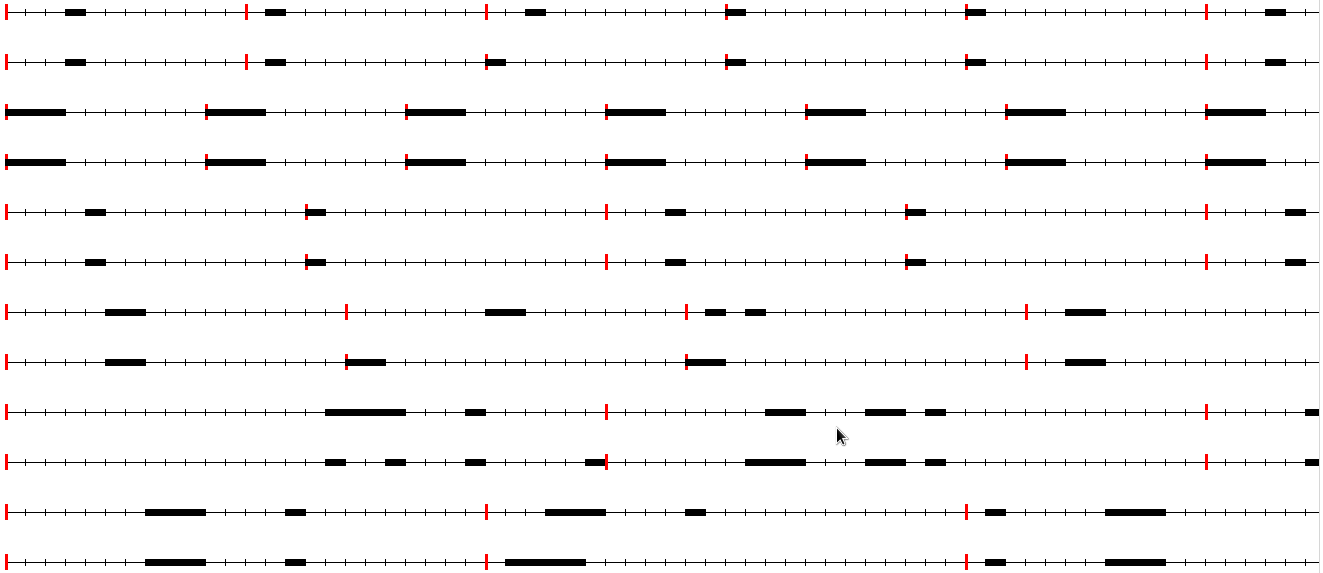
\includegraphics[width=\columnwidth]{fig/app2CheSc.png}
\end{figure}

\subsection{Aplicação 3}
A aplicação 3 foi projetada para que a sua utilização seja 100\%. O intuito de ter uma utilização igual a capacidade máxima é analisar se o algoritmo consegue utilizar todo o poder de processamento disponível. Podemos notar que o algoritmo de EDF continua escalonando normalmente e não tem perdas de \textit{deadlines}, já no RM há varias perdas de \textit{deadline} na tarefa 3.

\subsubsection{Código} 
\begin{lstlisting}[showstringspaces=false]
#include <hellfire.h>

void task(void){
	for(;;){
		printf("task %d \n", hf_selfid());		
		delay_ms(500);
	}
}
void app_main(void){
	hf_spawn(task, 10, 2, 10, "task 1", 1024);
	hf_spawn(task, 30, 5, 30, "task 2", 1024);
	hf_spawn(task, 50, 10, 50, "task 3", 1024);
	hf_spawn(task, 30, 6, 30, "task 4", 1024);
	hf_spawn(task, 30, 1, 30, "task 5", 1024);
	hf_spawn(task, 40, 8, 40, "task 6", 1024);
}
\end{lstlisting}

\subsubsection{Amostra do Escalonamento}

A Figura~\ref{fig:app3Hell} ilustra uma amostra do escalonamento gerado pelo HellfireOS, a Figura~\ref{fig:app3Chedder} mostra o escalonamento de dois processadores, um utilizando EDF e o outro RM. 

\begin{figure}[ht]
\centering
\caption{Aplicação 3 HellfireOS}
\label{fig:app3Hell}
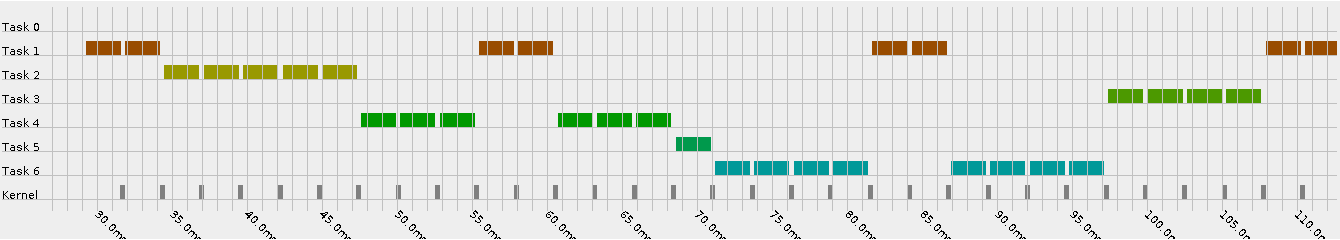
\includegraphics[width=\columnwidth]{fig/app3HellSc.png}
\end{figure}

\begin{figure}[ht]
\centering
\caption{Aplicação 3 Cheddar}
\label{fig:app3Chedder}
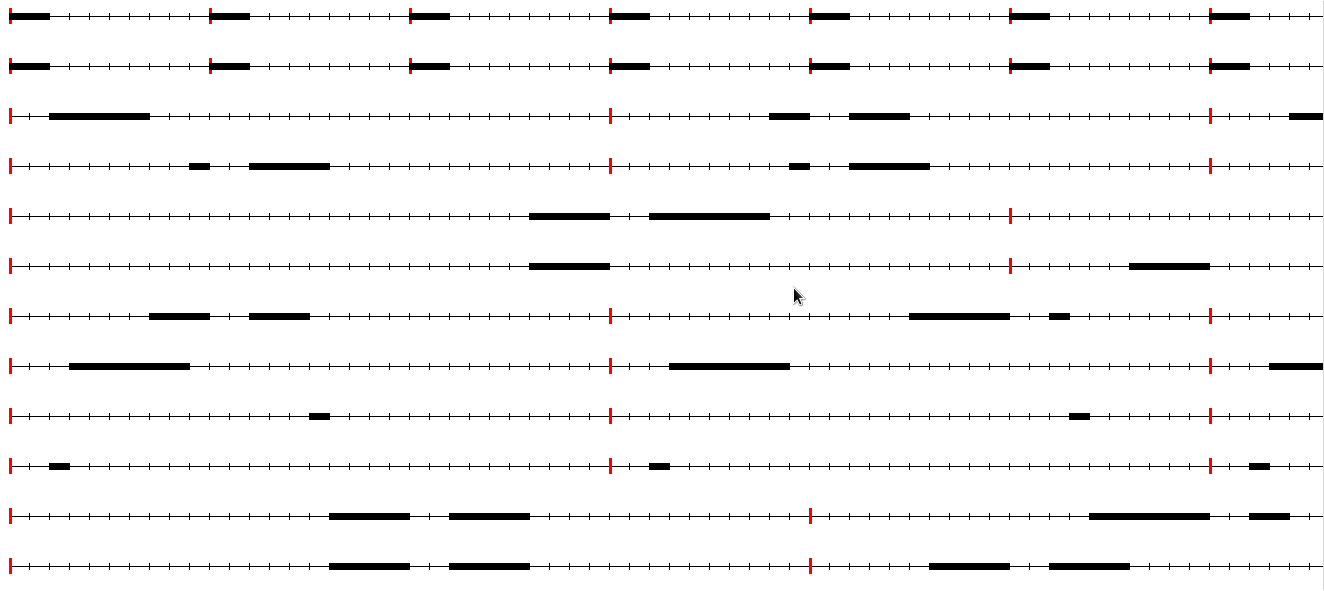
\includegraphics[width=\columnwidth]{fig/app3CheSc.png}
\end{figure}

\section{Dificuldades encontradas} 
Tivemos dificuldades no entendimento do funcionamento do HellfireOS na hora de analisar os resultados, pois como o simulador não mostra quando os \textit{deadline} irão acabar fica um pouco mais dificil de identificar. Ao contrário do que acontece na ferramenta Cheddar, onde o \textit{deadline} fica evidente e acusa quando acontecem perdas de \textit{deadline}. 

\section{Comentários finais} 

Como podemos analisar através das aplicações, o algoritmo RM não conseguiu escalonar tarefas com uma utilização maior que 90\%. Enquanto o EDF chegou a utilizar todo o processamento disponível, ou seja, 100\% da CPU. O EDF consegue explorar melhor os recursos computacionais e consegue ser mais responsivo a tarefas aperiódicas. 

Após pesquisar um pouco sobre os algoritmos, foi possível ver que sistemas embarcados que trabalham com recursos computacionais limitados e sistemas multimídias conseguem ser mais eficientes sobre um escalonamento EDF.

\end{document}
